\documentclass[conference]{IEEEtran}

\usepackage{amsthm}
\usepackage{graphicx}
\usepackage{amsmath}
\usepackage{algorithm}
\usepackage{algpseudocode}
\usepackage{listings}
\usepackage{color}
\lstset{language=c++,numbers=right,firstnumber=0,}
\newcommand{\RNum}[1]{\uppercase\expandafter{\romannumeral #1\relax}}


\newtheorem{definition}{Definition}
\newtheorem{theorem}{Theorem}
\newcommand{\todo}[1]{{\color{red}#1}}

\begin{document}

\title{A Projection-based Approach for Memory Leak Detection}
%---------
%\author{
%\IEEEauthorblockN{Xiaohui Sun\IEEEauthorrefmark{1},
							   %Sihan Xu\IEEEauthorrefmark{2}
%                               Chenkai Guo\IEEEauthorrefmark{2},
%                               Naipeng Dong\IEEEauthorrefmark{3},
%                               Quanqi Ye\IEEEauthorrefmark{6},
%                              Jing Xu\IEEEauthorrefmark{4},
%                              Xiujuan Ji\IEEEauthorrefmark{5}
%                            }
%                            \\
%\begin{tabular}{c c c c}                 
%    \IEEEauthorrefmark{5}Department of Binhai & \IEEEauthorrefmark{1}\IEEEauthorrefmark{2}\IEEEauthorrefmark{4}Department of Computer and Control Engineering & \IEEEauthorrefmark{3}\IEEEauthorrefmark{6}School of Computing\\
%    Nankai University & Nankai University & National University of Singapore &\\
%    \IEEEauthorrefmark{5}jixiujuan@mail.nankai.edu.cn & \IEEEauthorrefmark{1}2120150397@mail.nankai.edu.cn & \IEEEauthorrefmark{3}dcsdn@nus.edu.sg\\
%                                                      & \IEEEauthorrefmark{2}guochenkai88@gmail.com & \IEEEauthorrefmark{6}yequanqi@u.nus.edu\\
%                                                      & \IEEEauthorrefmark{4}xujing@nankai.edu.cn &
%\end{tabular}
%}
%------------------

%\author{
%\IEEEauthorblockN{Xiaohui Sun\IEEEauthorrefmark{1},
%                               Chenkai Guo\IEEEauthorrefmark{2},
%                               Naipeng Dong\IEEEauthorrefmark{3},
%                              Jing Xu\IEEEauthorrefmark{4},
%                              Xiujuan Ji\IEEEauthorrefmark{5}
%                            }
%\IEEEauthorblockA{\IEEEauthorrefmark{1,2,4}Department of Computer and Control Engineering, Nankai University}
%\IEEEauthorblockA{\IEEEauthorrefmark{3}School of Computing, National University of Singapore}
%\IEEEauthorblockA{\IEEEauthorrefmark{5}Department of Binhai, Nankai University}
%\IEEEauthorblockA{Email: \IEEEauthorrefmark{1} 2120150397@mail.nankai.edu.cn,
%\IEEEauthorrefmark{2}guochenkai88@gmail.com,
%\IEEEauthorrefmark{3}dcsdn@nus.edu.sg,
%\IEEEauthorrefmark{4}xujing@nankai.edu.cn,
%\IEEEauthorrefmark{5}jixiujuan@mail.nankai.edu.cn}}


%\author{
%\IEEEauthorblockN{Xiaohui Sun\IEEEauthorrefmark{1},
%                               Chenkai Guo\IEEEauthorrefmark{2},
%                               Naipeng Dong\IEEEauthorrefmark{3},
%                              Jing Xu\IEEEauthorrefmark{4},
%                              Xiujuan Ji\IEEEauthorrefmark{5}}\and
%\IEEEauthorblockA{\IEEEauthorrefmark{1}\IEEEauthorrefmark{2}\IEEEauthorrefmark{4}Department of Computer and Control Engineering\\
%    Nankai University\\
%\IEEEauthorrefmark{1}2120150397@mail.nankai.edu.cn\\
%\IEEEauthorrefmark{2}guochenkai88@gmail.com\\
%\IEEEauthorrefmark{4}xujing@nankai.edu.cn}
%\and
%\IEEEauthorblockA{\IEEEauthorrefmark{3}School of Computing\\
%    National University of Singapore\\
%\IEEEauthorrefmark{3}dcsdn@nus.edu.sg}
%\and
%\IEEEauthorblockA{\IEEEauthorrefmark{5}Department of Binhai\\
%    Nankai University\\
%\IEEEauthorrefmark{5}jixiujuan@mail.nankai.edu.cn}}

%\author{Xiaohui Sun}
%\affiliation{
%\institution{Department of Computer and Control Engineering, Nankai University}
%\city{Tianjin, China}
%\postcode{300350}
%}
%\author{Chenkai Guo}
%\affiliation{
%\institution{Department of Computer and Control Engineering, Nankai University}
%\city{Tianjin, China}
%\postcode{300350}
%}
%\author{Naipeng Dong}
%\affiliation{
%\institution{School of Computing, National University of Singapore}
%\city{Singapore}
%\postcode{117417}
%}
%\author{Jing Xu}
%\affiliation{
%\institution{Department of Computer and Control Engineering, Nankai University}
%\city{Tianjin, China}
%\postcode{300350}
%}
%\author{Xiujuan Ji}
%\affiliation{
%\institution{Department of Binhai, Nankai University}
%\city{Tianjin, China}
%\postcode{300350}
%}

\maketitle

\begin{abstract}
One of the major causes of software safety issues is memory leak; and the safety issues caused by memory leak are highly dangerous. Therefore, in order to ensure the software quality, memory leak detection is necessary. However, detecting memory leak vulnerabilities is challenging in source code analysis, as they are well concealed. Particularly, existing detection tools are weak in efficiency and accuracy especially when the targeted program contains a lot of branches with complex control flows. This paper proposes a projection-based approach to detect memory leaks in the C program's source code with multiple control flow branches. This approach projects the original control flow graph of a program to a simpler one according to the features of memory allocation and deallocation in C source code, which reduces the analysis complexity.  

This paper implements a memory leak detection tool PML\_Checker\protect\footnote{PML\_Checker.https://github.com/sunxiaohuiczcz/PML\_Checker.git.2017.} and evaluated the tool by comparing with the other three static detection tools like CppCheck on both public benchmarks and some new test cases provided by this paper. The detection results show that PML\_Checker reports the most memory leak vulnerabilities among other tools in C program's source code with complex control flow and complex data types, and PML\_Checker obtained higher efficiency and accuracy on public benchmarks.
\end{abstract}

%\keywords{ memory leak; projection algorithm; static analysis}

%!TEX root = bare_conf.tex
\section{Introduction}\label{sec:intro}
Memory leak is a major cause of reliability and performance issues in software. Especially in embedded systems, since it causes the long-running applications, which eventually will run out of memory. 
A system running out of memory may lead to the slowing down of the system caused by frequently swapping in and out, and process creation failure because of no more memory available. Moreover, memory leaks have caused severe consequences in some large applications and services. For example, on October 22, 2012, in the US-East region, a potential memory leak caused Amazon Elastic Block Store (EBS) and Elastic Compute Cloud (EC2) services to be six hours partially disrupted, and during this time services can not handle IO requests\footnote{ AWS Service Event.https://aws.amazon.com/cn/message/680342/.2017.}. 
Therefore, detecting memory leaks is very important and necessary to ensure the quality of software. Although memory leaks do not typically constitute a direct security threat, attackers can exploit them to increase a denial-of-service attack’s effectiveness.
However, detecting memory leaks is challenging, since the only symptom of memory leaks is the slow increasing of memory consumption.  

To address this challenge, there are two general techniques in existing works---dynamic testing and static source code analysis~\cite{AJ06}. 
Dynamic testing relies on the coverage of the test cases and requires long-time execution. Comparing to dynamic testing, static source code analysis has the advantage of higher accuracy, because static analysis is usually to find the memory allocation location and the corresponding release point.
%In fact, source code analysis is an important approach for detecting many vulnerabilities (including memory leaks) in software. 
Therefore, this paper focuses on detecting memory leaks by applying source code analysis.
Among source codes written in various languages, detecting memory leaks is particularly necessary when the program is written in low-level programming languages such as C/C++. Because low-level programming languages allow manual memory management, such as explicit memory allocation and deallocation~\cite{KJMP06}. Such manual memory operations are often error-prone, and even lead to vulnerabilities. 
%There has been previous related works on this problem~\cite{}.
%However, they become inefficient and less acurrate when complex control flows are involved. 

The relationship between memory allocation and deallocation can describe the root causes of memory leaks. In other words, the following two points show the classification of memory-leak reasons~\cite{LCW13}:(a)The dynamic memory blocks are not free/deallocated; (b)The dynamic memory blocks are freed in wrong order.
%\begin{itemize}
%\item[$\textbf{\emph{a.}}$]The dynamic memory blocks are not free/deallocated.
%\item[$\textbf{\emph{b.}}$]The dynamic memory blocks are freed in wrong order.
%\end{itemize}
To check the above two errors, there are in general the following two approaches: value-flow-based approach and control-flow-based approach. The basic idea of value-flow-based approach is to capture def-use chains and value flows, by assigning all memory locations represented by both top-level and address-taken pointers. Thence, it is also known as VFG (Value Flow Graph). While the basic idea of control-flow-based approach is to construct a dynamic memory allocation and deallocation model on the CFG (Control Flow Graph). Based on the CFG model, this paper checks whether a block of heap memory space is reclaimed by the program when the lifetime of the program has ended---if a block is not reclaimed, then there is memory leak. Comparing the VFG model~\cite{SYX12} with the projection-based CFG model, the latter focuses on all the possible execution paths, analyzes the lifetime of pointers that assigned memory locations. %We provide more detailed description for each type of memory leak in this model.
In particular, in order to capture the indirect allocation-deallocation relation and obtain accurate results.this paper takes into account the memory pointers' lifecycle, i.e., including all the memory operations.
 
The existing control-flow-based approaches have limitations in efficiency and accuracy when the control flow is getting complex, because the analysis of complex control flow needs to deal with a large number of path branches. %In this paper, we propose a concept named ``complex control flow'' in program analysis of memory leaks. 
We say that the control flow of a program is complex if the allocation and deallocation appear in different control flow branches of a program, and thus memory leaks are more likely to happen. Due to the complexity of the branch conditions' analysis, complex control flows make memory detection more difficult. %The complex control flow structures considered in this paper include the cases that the circulation complexity of a CFG (control flow graph) is not less than 2.
%Existing works have limitations  when the targeted program has complex control flows. 
In this work, this paper focuses on efficiently and accurately detecting memory leaks in programs with complex control flows.  
%The complexity of control flows of a program is closely related to the 
% the complexity of the program.
%The more complex the program is, the more complex the control flow of the program is.
%, and is also highly related to the number of software vulnerabilities. 
 
The higher complexity of the control flows is, the easier the vulnerabilities can hide. To detect memory leaks, detection system needs to search each control flow. Thus, the difficulty of detecting memory leaks in complex control flows increases with the complexity of paths in the control flows. Properly reducing the complexity of programs’ control flows can greatly improve the efficiency and accuracy of detecting memory leaks in the program. Therefore, in this work, this paper proposes to apply projection to the control flow grap. The projection abstracts the original control flow graph to a simplified graph to reduce the complexity of searching control flows in memory detection. The main challenge in the abstraction is to ignore the irrelevant paths. To address this challenge, when program has complex control flow branches, detecting system needs to evaluate the condition value of each control flow branch node, and then analyze the execution results of different branch paths according to different conditions. In order to achieve this goal, our system adopts path-sensitive analysis method~\cite{XA05}. This method records different program states of complex branch paths by tracing each branch of the program. This method analyzes the combinatorial relationship between branches. Thus the path-sensitive analysis method identify all the paths in a control flow graph. In other words, this method will abstract away some paths that are irrelevant to memory operations by matching the defined expression. A key issue in path-sensitive analysis is the evaluation of the guiding conditions of paths. To address this issue, our system uses a tool named PAT (Path Analysis and Testing)~\cite{ZW01}. PAT uses symbolic execution and constraint solving, to perform accurate evaluation on branch evaluations. %, but this two methods need sufficient time and space resources, and it is not suitable for more complex control flows analysis.
As a result, this paper proposes a set of rules for guiding the projection. Our approch essentially reduces irrelevant nodes in a control flow graph, and proves the correctness of the rules---no irrelevant path is considered and no relevant path is ignored.

%In order to achieve the accurate analysis for memory leaks in multiple control flow structures, in this paper, the idea of projection is applied to the analysis of control flow graphs. The abstract syntax tree is generated after the program lexical, syntax analysis. Our approach projects the original control flow graph to a simplified graph for reducing the analysis complexity based on abstract syntax tree. During the process of detecting memory leaks, we use the bottom-up approach to find bugs in the projection graphs.

The main contributions of this paper can be summarized as follows:
\begin{itemize}
\item The classification of memory leaks, particularly in source code with complex control flows.
\item A projection-based approach to detect potential memory leaks in C program, reducing the false negative rate in the program with complex control flows.
\item A detecting tool---PML\_Checker, evaluating the effectiveness and accuracy of the tool on public benchmarks (SPEC CPU 2000, SIR and SARD). 
\end{itemize}

In the next section this paper introduce our control flow graphs projection approach and prove its effectiveness. Section~\ref{sec:description} analyzes the causes of memory leaks and describe a leak model from the perspective of path-abstraction. Section~\ref{sec:approach} mainly presents the projection algorithm and memory leaks detection algorithm. In Section~\ref{sec:setup} and Section~\ref{sec:evaluation}, we conduct experiments to test PML\_Checker by comparing with three open-source detection tools, and we evaluate it at its effectiveness, accuracy, efficiency and scalability. Section~\ref{sec:related} discusses related research. And finally we conclude this work in Section~\ref{sec:conclusion}.

%!TEX root=bare_conf.tex
\section{Problem Description}\label{sec:description}
The targeted problem in this paper is the dynamic memory leaks - A block of heap memory space is being leaked if the program or the run-time system does not reclaim its memory when the lifetime of heap memory space has ended. 
The lifetime of heap memory space is represented in three ways in existing works~\cite{OR06}: 
\begin{itemize}
\item
\textit{Referencing:} the lifetime of a block of a heap memory space ends when there are no references to the space (excluding references from abandoned spaces).
\item 
\textit{Reachability:} the lifetime of a heap memory space ends when it is no longer reachable from program variables.
\item 
\textit{Liveness:} the lifetime of a heap memory space ends after the last access to that space.
\end{itemize}
In this paper, we focus on the second view - reachability, as reasoning on the reachability is more intuitive in the CFG, which our analysis is based on.
In the reachability view, there is a memory leak if the lifetime of a heap memory space ends while the memory pointer can not reach to that space.
%This paper analyzes the reasons for memory leaks from the perspective of control flow, which is based on the second way - reachability. 
Since our approach is based on CFG, detecting memory leaks is essentially analyzing whether the memory pointers have been freed when the lifetime of the corresponding memory spaces end in each branch of the control flow graph. Therefore, the memory detection can be converted into a control flow graph analysis on the correspondence relation between the memory pointers and the lifetime of the corresponding memory spaces, referred to as the reachability of the pointers.

As stated in Section~\ref{sec:intro}, when procedure $P$ has multiple control flow branches, the pointers pointing to corresponding memory spaces may be freed in wrong order, and the allocation and deallocation of memory space may appear in different control flow branches, this increases the complexity of the control flow graph analysis, because of the complex branch guarding condition analysis. %In addition, high control flow complexity will result in more difficult paths analysis. 
%The following definition defines the complex control flow.
We formally define the complex control flow as follows.

\begin{definition}[Complex Control Flow]
Given that a directed graph named $G= (N, E)$ is the control flow graph of a procedure $P$, where $N$ denotes the set of nodes and $E$ denotes the set of edges, the control flow is called \emph{complex control flow} when the cyclomatic complexity of $G$, denoted as $V(G)$, is no less than $2$. That is $V(G)=D+1\geq 2$, where $D$ denotes the number of conditional and loop branching nodes.
\end{definition} 

Fig.~\ref{fig:1} displays this generation of complex control flow. A simple control flow graph of procedure $P$ with memory allocation and deallocation is shown on the left. After adding the control flow branches, a complex control flow graph is shown on the right. Therefore, we need to analyze whether the memory spaces are released in each branch after being allocated. It should be noted that this section only considers the cases that allocate or release memory space of the same pointer, and the case that memory spaces are not fully released does not exist. There are four cases corresponding to the values of the two branches in the complex control flow graph:
\begin{enumerate}
\item
B1 =$\mathit{false}$, B2 = $\mathit{false}$: Corresponding to path 1-6-7. No memory leaks occur in this case, since there is no memory operations.
\item
B1 =$\mathit{true}$, B2 = $\mathit{false}$: Corresponding to path 1-2-3-7. The memory blocks have not been freed after being allocated, which is a typical kind of memory leaks.
\item 
B1 = $\mathit{false}$, B2 = $\mathit{true}$: Corresponding to path 6-4-5. The unallocated memory blocks are freed.
\item
B1 = $\mathit{true}$, B2 = $\mathit{true}$: Corresponding to path 1-2-3-4-5. Whether there is memory leak in this case is uncertain. The result relies on the number of executions of the memory allocation or deallocation related statements. Specifically, if both B1 and B2 are conditional branches, the memory allocation and deallocation will be executed only once, then there are no memory leaks in this structure. If B1 or B2 is a loop node, then the memory allocation or deallocation for the same pointer $p$ will be executed more than once in the loop, which will lead to a memory leak e.g., if B1 is a loop node, then multiple memory spaces are allocated, each in a single execution of the loop; but B2 is a conditional node, and thus there is only one deallocation in the branch. %In summary, the case that B1 =$\mathit{true}$ \&\& B2 =$\mathit{true}$ can be judged as memory leaks for the uncertainty of memory allocation and deallocation in static analysis.
\end{enumerate}

\begin{figure}[!h]
\center
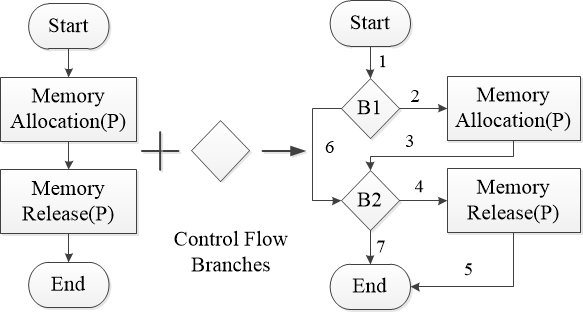
\includegraphics[width=0.45\textwidth]{figure/fig1-fig4/fig1}
\caption{Description of memory leaks reasons}
\label{fig:1}
\end{figure}

\begin{figure}[!h]
\center
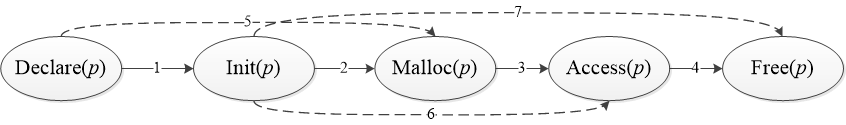
\includegraphics[width=0.45\textwidth]{figure/fig1-fig4/fig2}
\caption{Lifetime of a pointer $p$}
\label{fig:2}
\end{figure}

In each branch of the control flow graph, in addition to considering the allocation and deallocation of memory spaces, we need to additionally consider the lifetime of each pointer, as shown in the definition of dynamic memory leaks. To provide some clue, Fig.~\ref{fig:2} shows the lifetime of a pointer $p$ pointing to a heap memory space, using C language as an example. This figure shows the lifetime of a pointer $p$ from being declared to being freed. The solid arrows represent the correct order. The dotted arrows represent all the cases that may result in the memory leaks on the memory blocks refereed by a single pointer $p$. In details, the dotted arrow $5$ shows the case that the pointer $p$ is not initialized before being allocated to memory blocks, arrow $6$ illustrates that the pointer $p$ is not allocated to memory blocks before being accessed, arrow $7$ presents that $p$ is not allocated to memory blocks before being freed.

Note that Fig.~\ref{fig:2} only shows the lifetime of one pointer. When multiple pointers are considered, the cases that may lead to memory issues are complicated, which is another challenge in the memory leak detection.

%!TEX root=bare_conf.tex
\section{Approach}\label{sec:approach}
Similar to the CFG based static analysis, this paper also first constructs a detection model of C program, where memory leak may happen. The main difference of our approach is that, our approach performs projection in constructing the detection model, which simplifies the later memory leak detection procedure based on the model.

\subsection{Projection Algorithm}

This section describes a set of rules and an algorithm for projecting a control flow graph to a simply one. First of all, this paper introduces several concepts. These are going to be used in the projection rules.

%\begin{definition}[Projection Subject]
%Projection subject is the control flow graph of the program to be analyzed, which is a directed graph $G=(N, E)$, where $N = \{n_1, n_2, \ldots, n_k\}$ denotes the set of nodes, and $E = \{e_1, e_2, \ldots, e_k\}$ denotes the set of edges. In the procedure $P$, each statement is a node $n$, and there is an edge $e$ between two statements executed in sequence. 
%\end{definition}

Projection Subject is the input of the projection process and Projection Target is the output of the projection process. Specifically, Projection Subject($G$) is the control flow graph of the program to be analyzed. $G=(N, E)$, where $N = \{n_1, n_2, \ldots, n_k\}$ denotes the set of nodes, and $E = \{e_1, e_2, \ldots, e_k\}$ denotes the set of edges. In the procedure $P$, each statement is a node $n$, and there is an edge $e$ between two statements executed in sequence. Projection Target($G^*$) is a directed graph that contains all the control flow branch nodes denoted by $B$, and all the allocation nodes denoted by $A$ and deallocation nodes denoted by $F$ (if exist). $G^* = (N^*, E^*)$, where $N^* = A\cup B\cup F$ ($A\cap B\cap F=\emptyset$) denotes the set of nodes, and $E^*$ denotes the set of edges between nodes, representing the sequential ordering between nodes.

%\begin{definition}[Projection Target]
%Projection target is a directed graph $G^*$ that contains all the control flow branch nodes denoted by $B$, and all the allocation nodes denoted by $A$ and deallocation nodes denoted by $F$ (if exist). $G^* = (N^*, E^*)$, where $N^* = A\cup B\cup F$ ($A\cap B\cap F=\emptyset$) denotes the set of nodes, and $E^*$ denotes the set of edges between nodes, representing the sequential ordering between nodes.
%\end{definition}

\begin{definition}[Control Flow Graph Projection]
Given two directed graphs $G = (N, E)$ and $G^* = (N^*, E^*)$. Let set $M$ contains all the statement nodes relating to memory management in the procedure $P$ and the set $B$ contains all the control flow branch nodes (e.g. {\sf if}, {\sf else}, {\sf while}, {\sf for} et al.). If $G$ and $G^*$ satisfy the following conditions, then we say that $G^*$ is the projection of $G$, denoted as $G^* \mapsto G$:
\begin{itemize}
\item
$N^*\subseteq N$;
\item
If $\forall m,n\in N^*,(m\neq n), if m\in \Gamma(n)$ ($\Gamma(n)$ denotes the set of direct successor nodes of $n$), then there must be a connected path $\mu$ from $n$ to $m$ in $G$, formally $\exists \mu=(n, n_1,\ldots,n_l,m)$ in $G$ and $n_1\in\Gamma(n) \land  n_{i+1}\in\Gamma(n_i) \land n_n\in \Gamma(m)$ ($0\leq i\leq (n-1)$);
\item
$\forall$ $n\in B$ in directed graph $G^*$, if $\forall m\in M: m\not\in \Gamma(n)$, then $\Gamma(n)=\Gamma(n)\cup\{n\}$. 
\end{itemize}
\end{definition}

In general, the Control Flow Graph Projection is the process from the Projection Subject transforming into the Projection Target according to the following rules, we summarize the projection rules as follows: 
\begin{itemize}
\item 
Rule 1: The set $N^*$ of the projection graph only contains nodes related to memory allocation and deallocation, and all the control flow branch nodes in the procedure $P$.
\item
Rule 2: If a control flow branch contains the nodes related to memory allocation and deallocation, then the nodes that related to memory allocation and deallocation will be the successor nodes of this branch node in the projection graph $G^*$.
\item
Rule 3: If a control flow branch does not contain direct successor nodes that related to memory allocation and deallocation, then this branch node will form a closed node in the projection graph $G^*$. 
If the node $n\in N^*$, $n\in \Gamma(n)$, then the node $n$ is a closed node.
\end{itemize}


% that is, the degree of the branch node plus one.

Fig.~\ref{figure3} shows the CFG (G) of a piece of code. In this graph, there are $11$ elements forms set $N$, that is, $N = \{S_0, S_1, S_2, S_3, S_4, S_5, S_6, S_7, S_8, S_9, S_{10}\}$. The memory block is allocated in $S_1$ ($S_1\in A$) and freed in $S_9$ ($S_9\in F$); $S_3$ is a looping branch node and $S_6$ is a conditional branch node ($B=\{S_3, S_6\}$); In node $S_7$, another pointer points to the memory block ($S_7\in A$); Others are unrelated to memory operation. Thus the cyclomatic complexity of this graph is $4$.
Fig.~\ref{fig:4} shows the projection graph $(G^*)$ of $G$. Following the projection Rule 2, we have $N*=A\cup B\cup F=\{S_1, S_3, S_6, S_7, S_9\}$. Following Rule $2$, we have the edges from $S_1$ to $S_3$, $S_3$ to $S_6$, $S_6$ to $S_7$ and $S_7$ to $S_9$. Following Rule $3$, $S_3$ is a closed node since all its direct successor nodes are not memory related nodes, thus we add a loop to $S_3$. There is no loop at $S_6$, because the direct successor $s_7$ is a memory related node.  

\begin{figure}[!h]
\center
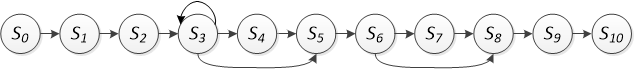
\includegraphics[width=0.5\textwidth]{figure/fig1-fig4/fig_3}
\caption{The CFG of the program (G)}
\label{figure3}
\end{figure}

\begin{figure}[!h]
\center
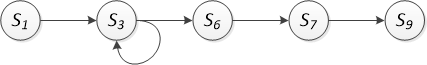
\includegraphics[width=0.35\textwidth]{figure/fig1-fig4/fig_4}
\caption{The projection graph (G*)}
\label{fig:4}
\end{figure}

\begin{theorem}[Control Flow Graph Projection Theorem]
Given a directed graph $G = (N, E)$. If $G^* \mapsto G$ where $G^*=(N^*, E^*)$, then $G^*$ strictly keeps the reachability relation among nodes in $N^*$ from $G$, that is, $\forall m,n\in N^*$, $m$ can reach $n$ in $G^*$ if and only if $m$ can reach $n$ in $G$.
\end{theorem}

\begin{proof} Presume $m$ can reach $n$ in $G^*$, which means there exists a directed path $\mu^*=(m,e_1^*,e_2^*,\ldots,e_k^*,n)$ in $G^*$. 
Since $G^* \mapsto G$, then there must exist a set of paths $\mu_0=(m,e^0_i,\ldots,e^0_{j_0}, e_1^*)$, $\mu_i=(e^*_{i}, e^{i}_i,\ldots,e^{i}_{j_i}, e_{i+1}^*)$ ($1\leq i\leq k-1$) and $\mu_k=(e_k^*,e^k_i,\ldots,e^k_j, e_{j_k}, n)$ in $G$, where $e^{i}_{j_i}$ can be empty. The $k$ paths are connected since the last node in a path is the starting node of another path. Formally, given path $\mu_i=(e^*_{i}, e^{i}_i,\ldots,e^{i}_{j_i}, e_{i+1}^*)$ and $\mu_{i+1}=(e^*_{i+1}, e^{i+1}_{i+1},\ldots,e^{i+1}_{j_{i+1}}, e_{i+2}^*)$. According to the definition of path, we have $e_{i+1}^*\in \Gamma(e^{i}_{j_i})$ in path $\mu_i$
and $e^{i+1}_{i+1} \in \Gamma(e^*_{i+1})$ in path $\mu_{i+1}$. Thus we have a path from $e^{i}_{j_i}$ to $e^{i+1}_{i+1}$ via $e^*_{i+1}$. That is we can connect $\mu_i$ and $\mu_{i+1}$ as path $(e^*_{i},e^{i}_i,\ldots,e^{i}_{j_i}, e_{i+1}^*, e^{i+1}_{i+1},\ldots,e^{i+1}_{j_{i+1}}, e_{i+2}^*)$. In this way, by connecting the $k$ paths, we have a path from $m$ to $n$ in $G$.
%At the same time, then there must exist $\mu=(e_j^*,\ldots,e_t^*)\in G$ for $e_j^*, e_t^*\in μ^* (1\leq j<t\leq k)$ , $e_t^*\in \Gamma(e_j^*)$. So on and so forth, the directed path $\mu=(n,\ldots,m)\in G$ can be deduced, that is $m$ can reach $n$ in $G$. 

On the other hand, presume $m$ can reach $n$ in $G$, that is there exists a directed path $\mu=(m,\ldots,n)$ in $G$, then there must be:
\begin{itemize}
\item
Either there are no other nodes in $N^*$ except $m$ and $n$; 
\item
Or there is $\mu=(m,\ldots,n_1,\ldots,n_2,\ldots,n_k,\ldots,n)$, where $m$, $n$, $n_i\in N^* (1\leq i \leq k)$, and the remaining nodes do not belong to $N^*$.
\end{itemize}
%
In the former case, according to the rules of control flow graph projection, $m$ can immediately reach $n$ in $G^*$, i.e., $n\in \Gamma(m)$.
%
In the later case, let $\mu=m,\mu_1,n_1\mu_2, n_2,\cdots,\mu_k, n_k, \mu_{k+1}, n$, where $\mu_i=(n^i_{1},\ldots,n^i_{j_i}) (1\leq i\leq k+1)$, there are no nodes in each path $\mu_i$ from $N^*$ except end nodes. According to the projection rules, the nodes in each path $\mu_i$ will be deleted in $G^*$ such that there is a immediate edge between $m$ and $n_1$, between each $n_i$ and $n_{i+1} (1\leq i \leq k)$, and between $n_{k+1}$ and $n$, which forms a path $
\mu^*=(m, n_1, n_2, \ldots, n_{i}, n_{i+1}, \ldots, n_{k+1}, n)$ in $G^*$. 
\end{proof}

Algorithm~\ref{alg:cfp} shows the projection algorithm according to the projection rules. %We can summarize from the control flow graph projection theorem that $G^*$ is a directed graph extracted from $G$ which consists of $N^*$. Apart from this, $G^*$ strictly keeps the reachable relationships among nodes in $N^*$ from $G$. Specifically, if $N^* = N$, then $P[G, N^*] = G$.
%
Given the control flow graph $G = (N, E)$ of program $P$ as input. The algorithm returns $G$'s projection graph $G^*= (N^*, E^*)$ as output. Algorithm 1 can be divided into $3$ steps. Step$1$(line $1-2$) establishes the min-heap of $N$ according to the execution order of statements. Step$2$(line $3-9$) folds those unrelating to memory management paths. Step$3$(line $10-12$) adjusts the $\mathit{Red\_Black\_Tree}(N^*)$ and the $\mathit{Map}(N^*)$, and obtains the final projection graph $G^*$).
% and $G^*=P[G, N^*]$. $N^* = A\cup B\cup F$. Moreover, 
In this algorithm, $n.ind$ and $n.outd$ stand for the in-degree and out-degree of node $n$ respectively. $A.a$ means the node $a$ is in set $A$. $F.f$ means the node $f$ is in $F$. Lastly, whenever a loop is added to $G^*$ (even when the loop already exists), both the in-degree and the out-degree of the looping node are increased by one.

%The set $N$ contains all the nodes abstracted from the statements from procedure $P$. 
Considering the complexity of the projection algorithm, the Red Black Tree is used to store the nodes in set $N$. Red Black Tree is a data structure, which is an approximate balanced tree with only two types of nodes: red nodes and black nodes. This type of data structure has the advantage of high search efficiency, due to that it is sequential which can avoid the disorder during the search process. 

In the algorithm, the set $E$ in graph $G$ (the execution sequence of statements in procedure $P$) is implemented as a set of $Map$s. A $Map$ is a data structure stored in the form of key-value pairs. The elements in a $Map$ are the ordering relation between a node $n$ in set $N$ and its successor nodes (i.e., nodes in $\Gamma(n)$).

\begin{algorithm}
\caption{ControlFlowProjection ($G$)}\label{alg:cfp}
\textbf{Input:} A control flow graph $G$ for program $P$.\\
\textbf{Output:} Projection graph $G^*$ for the input control flow graph\\
%\textbf{Begin}\\
%Step1: (According to the execution order of statements, establish the min-heap of $N$)\\
1.\quad	Initialize the Red Black Tree $\mathit{Red\_Black\_Tree}(N)$.\\
%2.\quad	\textbf{init} $\mathit{Red\_Black\_Tree}(N)$;\\
%3.\quad	\textbf{create} $\mathit{Red\_Black\_Tree}(N)$;\\
%2.\quad	$\forall n\in N, \mathit{Map}(n)\leftarrow(n,\Gamma(n))$;\\
2.\quad	For all $n$ from $N$, add $n$ and $\Gamma(n)$ to $\mathit{Map}(n)$.\\
%Step2: (Fold paths)\\
3.\quad	\textbf{while} $\mathit{Red\_Black\_Tree}$.hasNext \textbf{do}\\
%4.\quad	\textbf{do}\\
4.\quad	\textbf{if} $n.ind\geq 2 || n.outd\geq 2$ \textbf{then}\\
5.\quad \quad    \textbf{if} $A.a\in \Gamma(n) || F.f\in \Gamma(n)$ \textbf{then}\\
6.\quad \quad	   $\Gamma(n)\leftarrow A.a || \Gamma(n)\leftarrow F.f$.\\
7.\quad	\textbf{else then} \\
8.\quad \quad  $\Gamma(n)\leftarrow (n\cup \Gamma(n)\cap N^*)$.\\
9.\quad\textbf{end while}\\
%Step3: (Adjust the $\mathit{Red\_Black\_Tree}(N^*)$ and the $\mathit{Map}(N^*)$, and obtain the final projection graph $G^*$)\\
10.\quad	Delete all $n$ that are not in $N^*$.\\
11.\quad	$\mathit{Red\_Black\_Tree(N)} \leftarrow \mathit{Red\_Black\_Tree}(N^*)$.\\
12.\quad	$\mathit{Map}(N) \leftarrow \mathit{Map}(N^*)$.\\
%\textbf{End}
\end{algorithm}

The projection algorithm is acceptable in the aspect of complexity. In this algorithm, this paper assumes that the number of edges is linear in N, all the time complexity of Step1, Step2 and Step3 are $O(log(N))$, and the space complexity of the three steps are $S(N)$($S(N)$ is linear). Therefore, the time complexity of this algorithm is $O(log(N))$ and the space complexity of this algorithm is $S(N)$.

\subsection{Detection Method}

%$G^* \mapsto G$, and $G^*$ is the projection graph of the control flow graph $G$, and there are two definitions on $G^*$.
Given a graph $G^*=(N^*, E^*)$, this paper defines the direct predecessor of a node as follows:

\begin{definition}{Direct Predecessor Node}
For two nodes $m$, $n$ ($m, n\in N^*$), if $m$ is the first open node among all the predecessor nodes of node $n$ (i.e., $Η(n)$), then $m$ is called the direct predecessor node of $n$.
\end{definition}

The detection algorithm (Algorithm~\ref{alg:mld}) takes the output of the projection process as input. %In this paper, stack elimination\footnote{Eliminating Frame Pointer and Arg Pointer. http://gcc.gnu.org/onlinedocs/gccint/Elimination.html. 2017.} is leveraged to detect memory leaks in source code. Algorithm~\ref{alg:mld} shows the detection algorithm, 
Given the nodes in set $A$ or $F$, the algorithm finds the direct predecessor node of all nodes by traversing the Red Black Tree. In this algorithm, the node $base$ is the last node in set $A$ or $F$ traversed to, i.e., $base$ is the currently visiting node. In line $7-12$, the first node from $A$ or $F$ will be pushed into the stack when the stack is empty. Otherwise it traverse the next node. In line $14-20$, there may be memory leaks when the direct predecessor node of $base$ is the node from $B$, according to the second case from Fig.~\ref{fig:1} in Section~\ref{sec:description}. Another situation is that the direct predecessor node of base is not the node from $B$, if the stack is not empty after the detection process, then there may be some memory spaces that have not been freed which may lead to memory leaks.

\begin{algorithm}
\caption{MemoryLeakDetection ($G^*$)}\label{alg:mld}
\textbf{Input:} The projection graph $G^*$.\\
\textbf{Output:} The detection results for memory leaks ($\mathit{true}$ or $\mathit{false}$)\\
%\textbf{Begin}\\
1.\ \	Declare a $\mathit{stack}$ to be detected.\\
2.\ \ 	Declare node $\mathit{base}$ and node $\mathit{current}$ for traverse.\\
3.\ \        $\mathit{Check\_MemLeak}$(Tree $\mathit{Red\_Black\_Tree}$, Set $\mathit{Map}$)\\
4.\ \ 	\textbf{while} $\mathit{Red\_Black\_Tree}$.hasNext \textbf{do} \\
%5.\ \ 	\textbf{do begin}\\
5.\ \quad	   set $\mathit{base} =$ null.\\
6.\ \quad	   set $\mathit{current} = \mathit{Red\_Black\_Tree}$.$\mathit{current\_Ele}$\\
7.\ \ \quad	    \textbf{if} $\mathit{base}$ == null \textbf{then}\\
8.\ \ \quad\quad	        \textbf{if} $\mathit{current}$ != $A$ \&\& $\mathit{current}$ != $F$ \textbf{then}\\
9.\ \ \quad\quad\quad	            \textbf{continue}.\\
10.\ \ \quad\quad	        \textbf{else then}\\
11.\ \ \quad\quad\quad	            $\mathit{base} \leftarrow \mathit{current}$.\\
12.\ \ \quad\quad\quad	            $\mathit{stack}$.push($\mathit{base}$).\\
13.\ \ \quad	    \textbf{else then}\\
14.\ \ \quad\quad       \textbf{if} $\mathit{current}\in B$ \textbf{then}\\
15.\ \ \quad\quad\quad            \textbf{if} $B.ind<2 || B.outd<2$ \textbf{then}\\
16.\ \ \quad\quad\quad\quad	                \textbf{return} $\mathit{false}$.\\
17.\ \ \quad\quad\quad        \textbf{else if} $\mathit{current} == \mathit{base}$ \textbf{then}\\
18.\ \ \quad\quad\quad\quad	            $\mathit{stack}$.push($\mathit{current}$).\\
19.\ \ \quad\quad\quad	        \textbf{else if} $\mathit{current}$ != $\mathit{base}$ \textbf{then}\\
20.\ \ \quad\quad\quad\quad	            $\mathit{stack}$.pop().\\
21.\ \ 	\textbf{end while}\\
22.\ \ 	\textbf{if} $\mathit{stack}$ != null \textbf{then}\\
23.\ \ \quad    \textbf{return} $\mathit{false}$.\\
24.\ \ 	\textbf{else then}\\
25.\ \ \quad	    \textbf{return} $\mathit{true}$.\\
%\textbf{End}
\end{algorithm}

There are only one loop in the traversal of Red Black Tree, so the time complexity of this algorithm is $O(log(N))$, and the space complexity of this algorithm is $S(N)$.

Take projection graph in Fig.~\ref{fig:4} as an example. According to the detection algorithm, the direct predecessor node of node $S_9$ is node $S_7$, and the direct predecessor node of node $S_7$ is node $S_6$, node $S_6$ is a branch node. That is, the memory blocks are freed in the conditional branch of node $6$, which is determined to be a suspected memory leak.

\subsection{Optimization Strategy}

The control flow graph projection makes the detection process simple and intuitive. More importantly, all the cases of memory leaks mentioned in Section~\ref{sec:description} can be detected in the detection algorithm. However, this approach may result in a high false positive rate, since it does not analyze the specific value of conditional predicate in the valuating of control flow branches, which leads to a low sensitivity to data flows. In Fig.~\ref{fig:7}, the statement $5$ will be marked with a $B$ node (control flow branching statement). Apart from this, the example code will be judged to have a suspected memory leak, by using the algorithm above, since the buffer may not be freed in every branch. However, there are no memory leaks in this example. Specifically, the result of the condition is true when analyzing the conditional predicate of line $5$ (buffer != NULL), that is, the memory blocks are freed after being allocated. 

In order to reduce such false positives, this paper combines symbolic execution\footnote{Symbolic execution.https://en.wikipedia.org/wiki/Symbolic\_execution.2017.} and constraint solving\footnote{Constraint solving. http://www.constraintsolving.com/. 2017.} during the execution of the algorithm to accurately evaluate the branching conditions.
%
\begin{figure}[!h]
\small
\center
\begin{lstlisting}[frame=single,framexrightmargin=-10pt,numbers=right] 
void main(){
 long *buffer;
 size_t size;
 buffer= (long*)malloc(1000*sizeof(long));
 size = _msize(buffer);
 if(buffer != NULL)
 free(buffer);
}
\end{lstlisting}
\caption{A piece of code}\label{fig:7}
\end{figure}

Symbolic execution simulates the execution of programs by symbolizing variables. Specifically, symbolic execution collects memory allocation and release points by backward traversal for the CFG. At the same time, at each of the control flow branch, conditions of the branch are added to the current path conditions. Finally, those paths related to memory allocation and release will be merged at the meeting node of the CFG, and then according to Hoare logic\footnote{Hoare logic. https://en.wikipedia.org/wiki/Hoare\_logic. 2017.}, our system carries constraint solving to the merged paths. Constraint solving is accompanied by the projection process.  
%Therefore, symbolic execution and constraint solving can help to reduce similar false positives like the problem in this example.

\subsection{System Workflow}

%\begin{figure}[!h]
%\small
%\centering
%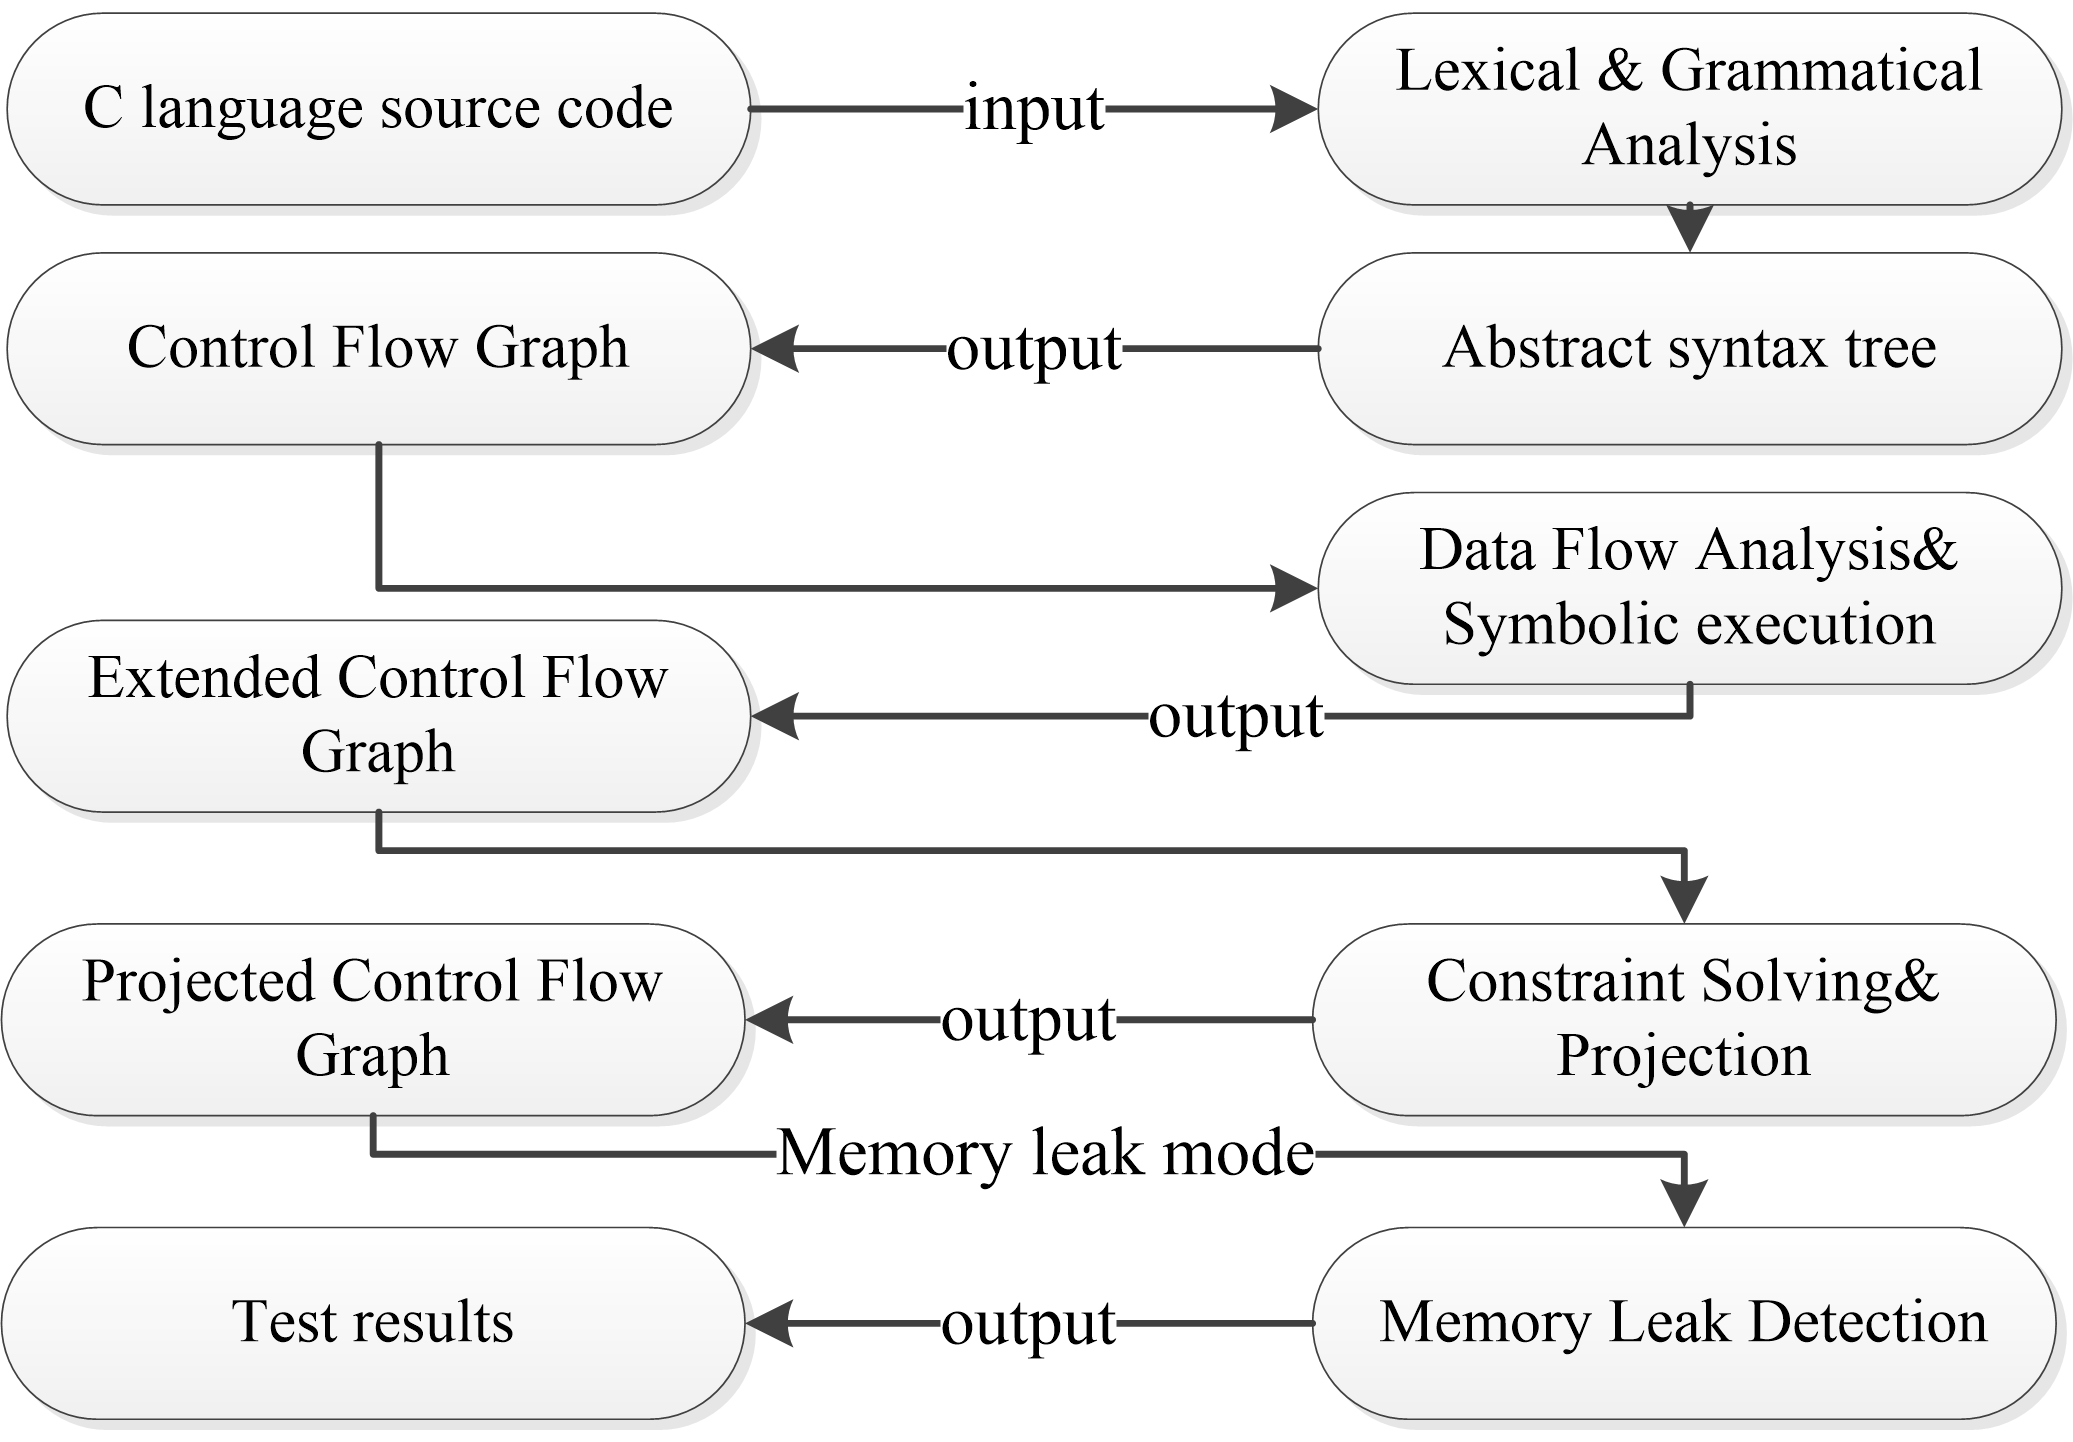
\includegraphics[width=0.5\textwidth]{figure/fig8-fig12/fig_new}
%\caption{Framework flowchart for PML\_Checker}\label{fig:18}
%\end{figure}

The input data of PML\_Checker is C language source code. After lexical analysis and syntax analysis, abstract syntax tree generates the original control flow graph, which will be output to the system interface. Next, data flow analysis and symbolic execution extend the original CFG, constraint solving to the data flow conditions will find the dependencies from the memory allocation to deallocation, and the extended CFG will be output as a mid product. Then the projected CFG wil be produced at the base of extended CFG by projection algorithm. At last, according to the detection method mentioned at the approach section, PML\_Checker detects memory leaks from the projected CFG, and displays the test results. 


%!TEX root=bare_conf.tex
\section{Experiments}\label{sec:experiments}

To evaluate the projection approach proposed in Section~\ref{sec:approach}, 
%we experimentally compare our approach and existing approaches for memory leak static analysis. We 
this paper compares our tool -- PML\_Checker with other tools which represent the existing different static detection approaches. 

In general, this paper investigates the following research questions in the following experiments:
\begin{description}
\item[RQ1:] How does our approach perform compared with existing approaches in terms of effectiveness analysis for complex control flows? 
\item[RQ2:] How does our approach perform compared with existing approaches in terms of effectiveness analysis for complex data types? 
\item[RQ3:] How does our approach perform compared with existing approaches under the public benchmarks in terms of accuracy and run time analysis? 
\end{description}

\subsection{Experimental Setup}
In the rest of this section, this paper presents detailed information of the test subjects (Section~\ref{ssec:ts}), selected approaches to compare with (Section~\ref{ssec:ca}), the parameters and metrics (Section~\ref{ssec:pm}) in our experiments.

\subsubsection{Test Subjects}\label{ssec:ts}
For the sake of fairness, in the results of our experiments, this paper considers the effectiveness of the approach from two aspects: complex control flows and complex data types. In details, a complex control flow refers to a control flow graph with more than one control flow branches. Complex data types include data structure like linked list, struct, array and the combination of these data types. Furthermore, this experiment adopts all the C programs from SPEC CPU 2000\footnote{SPEC. http://www.spec.org/cpu/. 2007.}, SIR\footnote{SIR. http://sir.unl.edu/content/sir.php. 2017.} (Software-artifact Infrastructure Repository) and $40$ test cases about memory errors from the SARD\footnote{NIST. https://samate.nist.gov/SARD/. 2016.} (Software Assurance Reference Dataset) for measuring the accuracy of the projection approach. This paper presents on a number of small programs with memory leaks that have different complex control flows and complex data types. (Relevant test code can be accessed in footnote 1).
\subsubsection{Selected Approaches}\label{ssec:ca}
Table~\ref{tab:1} lists the $4$ approaches considered in our experiments. There are several reasons for selecting the following approaches and the corresponding tools. 
%
\begin{table}[!h]
\center
\caption{Information of approaches}\label{tab:1}
\begin{tabular}{|c|c|c|c|}
\hline
\textbf{No.} & \textbf{Abbreviation} & \textbf{Description} & \textbf{Tool}\\
\hline
A1 & exp-mat & expression matching & CppCheck\\
\hline
A2 & stl-not & style and notation &	Splint\\
\hline
A3 & steam-slic & resources streamlined slices & RL\_Detector\\
\hline
A4 & pro-grap &	CFG projection &	PML\_Checker\\
\hline
\end{tabular}
\end{table}
%
Regular matching and style, notation based detection are common approaches adopt in source code static detection. Both CppCheck\footnote{CppCheck. trac.cppcheck.net/wiki. 2016.} and Splint\footnote{Splint. http://www.splint.org/. 2010.} are open source static detection tools used in Windows operating system. Apart from this, both tools can detect memory leaks in C programming language. In details, Splint develops different detecting standards for different types of errors in the compilation process, it detects memory leaks by annotations to record the pointer object’s lifetime~\cite{EL02}. CppCheck first creates symbol database of variables, functions and so on, and then it detects memory leaks by the embedded inspection classes.
 
RL\_Detector is a static detection tool implemented, which adopts resources streamlined slices construction and is achieved a comparative accurate analysis of memory leaks. This section compares our tool PML\_Checker which implements the presented approach with the above tools.

\subsubsection{Parameters and Metrics}\label{ssec:pm}
There are some parameters and metrics used in our experiments for evaluation.
\begin{itemize}
\item \textit{TW:} The total number of the reported memory leaks.
\item \textit{TL:} The total number of memory leaks contained in a program, and it takes the number of pointers pointing to memory blocks as the measurement standard.
\item \textit{FP:} The number of false positives.
\item \textit{MLF:} The difference of \textit{TW} and \textit{FP}, which denotes the number of real memory leaks in the test results.
\item \textit{FPR:} The false positive rate, a metric used to measure the accuracy. It can be calculated by the following formula: \textit{FPR}=$\frac{\textit{FP}}{\textit{TW}}$.
\item \textit{FNR:} The false negative rate, a metric used to measure the accuracy. It can be calculated by the following formula: \textit{FNR}=1-$\frac{\textit{TW}}{\textit{TL}}$.
\item \textit{Time:} The run time of each tool for C program.
\end{itemize}

\subsection{Experimental Results}

\noindent RQ1: \textit{Effectiveness Analysis of Complex Control Flow}

The first research question is to compare the effectiveness achieved by the $4$ tools with respect to complex control flows. Table~\ref{tab:2} lists the test results on $9$ small programs and Fig.~\ref{fig:8} shows the number of the $4$ tools reported memory leaks in each control flow structure. Comparing our approach with other approaches, we have the following observations.

\begin{table}[!h]
\center
\caption{Test results on complex control flows}\label{tab:2}
\begin{tabular}{|c|c|c|c|c|c|}
\hline
\textbf{Test Case No.} & \textbf{Test Cases} & \textbf{A1} & \textbf{A2} & \textbf{A}3 & \textbf{A4}\\
\hline
C\_case1	& Simple\_branch &	YES & NO & YES & YES\\
\hline
%C\_case2 & Simple\_branch\_2 & \textendash & \textendash & \textendash & \textendash\\
%\hline
C\_case2	& Simple\_loop\_1 & NO &	NO & YES & YES\\
\hline
C\_case3	& Simple\_loop\_2	& YES &	NO & YES & YES\\
\hline
C\_case4	& Chain\_branch\_1 & NO & NO & YES & YES\\
\hline
C\_case5	& Chain\_branch\_2 &	NO	& NO & YES & YES\\
\hline
C\_case6	& Chain\_loop\_1 & YES & YES & NO & YES\\
\hline
C\_case7	& Chain\_loop\_2 & YES & YES & NO & YES\\
\hline
C\_case8	& Nesting\_branch & NO & NO & YES & YES\\
\hline
C\_case9 & Nesting\_loop & NO & NO & YES & YES\\
\hline
\multicolumn{2}{|c|}{FNR} & 56\% & 78\% & 22\% & 0\\
\hline
\end{tabular}
\end{table}

\begin{figure}
\center
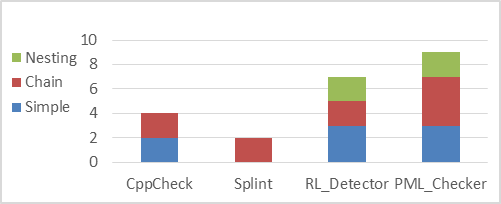
\includegraphics[width=0.45\textwidth]{figure/fig8-fig12/fig8}
\caption{Description of memory leaks reasons}
\label{fig:8}
\end{figure}

%First, all the $4$ tools did not detect the memory leak in C\_case2, because the memory leaks in C\_case2 are caused by allocating memory blocks in conditional branches. In this case, the program will be compiled failed, because the pointer pointing to memory blocks is not found during the execution of function ``free()". Therefore, this type of test case is often ignored in static analysis.

%First, we calculated the \textit{FNR} of the test results. In details, the false negative rate of CppCheck test results, that is \textit{FNR}(CppCheck) is 5/9 $\approx$ 0.56. In the same way, \textit{FNR}(Splint) = 0.78, \textit{FNR}(RL\_Detector) = 0.22, while \textit{FNR}(PML\_Checker) = 0. For the reason that the analysis method of PML\_Checker is based on the complex control flow, the results of PML\_Checker covered all the test cases about complex control flow in this experiment. In other words, the false negative rate of the CFG projection approach is lower than other approaches for detecting memory leaks in complex control flow, which reflects the effectiveness of this approach for complex control flow.

First, PML\_Checker covered all the test cases about complex control flow in this experiment. In other words, the \textit{FNR} of the CFG projection approach is lower than other approaches for detecting memory leaks in complex control flow, which reflects the effectiveness of this approach for complex control flow.

Second, regarding the comparison of the approaches, the regular match based approach compares the source code with the vulnerabilities in the process of detecting memory leaks. This approach is not sensitive to complex control flow and inflexible in the types of vulnerabilities to compare with. The style and notation based approach improves the software quality by improving the programming style and discovering the potential bugs that impacting the portability of programs. However, the memory leak analysis is not complete, so it has a high false negative rate. The approach by constructing resources streamlined slices only makes a simple assumption for allocation and deallocation of resources within loop bodies. It reduces the number of loops to 1 and treats the loops the same as branches. Therefore, this approach can not pass the test cases on the Chain\_Loop structure (C\_case6 and C\_case7) in the experiment.

\noindent RQ2: \textit{Effectiveness Analysis of Complex Data Flow}

The second research question is to compare the effectiveness achieved by the $4$ approaches with respect to complex control flows. Table~\ref{tab:3} lists the test results on $10$ small programs and Fig.~\ref{fig:9} shows the comparison on the number of  memory leaks in each data type by the $4$ tools. Comparing our approach with other approaches, we have the following observations.

\begin{table}[!h]
\center
\caption{Test results on complex data types}\label{tab:3}
\begin{tabular}{|c|c|c|c|c|c|}
\hline
\textbf{Test Case No.} & \textbf{Test Cases} & \textbf{A1} & \textbf{A2} & \textbf{A3} & \textbf{A4}\\
\hline
T\_case1	& Array\_1 &	YES & NO & YES & YES\\
\hline
T\_case2 & Array\_2 & NO & NO & NO & NO \\
\hline
T\_case3	& Array\_3 & NO &	NO & NO & YES\\
\hline
T\_case4	& List\_1	& NO &	NO & NO & NO\\
\hline
T\_case5	& List\_2 & NO & YES & NO & YES\\
\hline
T\_case6	& List\_3 &	NO	& YES & NO & YES\\
\hline
T\_case7	& Struct\_1 & NO & YES & NO & YES\\
\hline
T\_case8	& Struct\_2 & NO & YES & NO & YES\\
\hline
T\_case9	& Array\_struct\_1 & NO & YES & YES & YES\\
\hline
T\_case10 & Array\_struct\_2 & YES & YES & YES & YES\\
\hline
\multicolumn{2}{|c|}{FNR} & 80\% & 40\% & 70\% & 20\%\\
\hline
\end{tabular}
\end{table}

\begin{figure}[!h]
\center
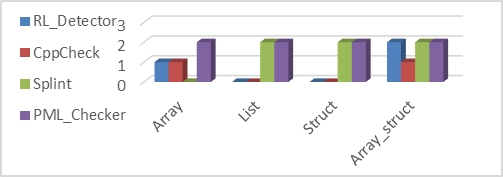
\includegraphics[width=0.45\textwidth]{figure/fig8-fig12/fig9}
\caption{The leaks number of each data type}
\label{fig:9}
\end{figure}

%First, the common high FNR shows us the accuracy of pointer alias analysis on complex data flow is relatively lower for all the tools.

First, the results of Splint and PML\_Checker show a higher effectiveness compared with the other two tools in the experiment. Splint has a high effectiveness because it mainly checks the specifications in programs, which is sensitive to different data types. Splint has a high effectiveness because it simplifies the analysis for complex data types in the process of abstracting the control flows. 

Second, comparing PML\_Checker with Splint, Splint reported memory leaks on the latter three data types (linked list, struct and array\_struct), except the memory leaks in an array in Fig.~\ref{fig:9}. Due to the programs that are provided in this paper are in small scale and simple data relationships, PML\_Checker shows a little advantage compared to Splint. For the former approaches, that is CppCheck and RL\_Detector, there is a large space to improve in analyzing the complex data types.

\noindent RQ3: \textit{Accuracy and Run Time Analysis of Benchmarks}

The third research question is to compare the accuracy achieved by the $4$ approaches, and the run time recorded by the corresponding $4$ tools in terms of open benchmarks. There are two experiments.

\noindent\textbf{Experiment on SPEC CPU 2000 and SIR} 
\\
This experiment analyzed the test results and run time of the four tools on SPEC CPU $2000$ and SIR, and the \textit{FPR} was selected to measure the accuracy of different approaches on the same test suite. Table~\ref{tab:4} shows the test results on SPEC CPU $2000$ and Table~\ref{tab:5} shows the test results on SIR. Compare our approach with other approaches, we have the following observations. 

%First, we calculate the false positive rates in Table~\ref{tab:4}, i.e., \textit{FPR}(CppCheck) =$ 2/19$ $\approx$ 0.11. \textit{FPR}(Splint) = 0.44. \textit{FPR}(RL\_Detector) = 0.09. \textit{FPR}(PML\_Checker) = 0.13. Similarly, in Table~\ref{tab:5}, \textit{FPR}(CppCheck) = 0.19, \textit{FPR}(Splint) = 0.30, \textit{FPR}(RL\_Detector) = 0.08, \textit{FPR}(PML\_Checker) = 0.18.

\begin{table}[!h]
\center
\caption{Test results on SPEC CPU $2000$}\label{tab:4}
\hspace{-0.5cm}\begin{tabular}{|c|c|c|c|c|c|c|c|c|c|}
\hline
& \textbf{Size} & \multicolumn{2}{|c|}{\textbf{A1}} & \multicolumn{2}{|c|}{\textbf{A2}} & \multicolumn{2}{|c|}{\textbf{A3}} & \multicolumn{2}{|c|}{\textbf{A4}}\\
\hline
Program & Kloc & TW & FP & TW & FP & TW & FP & TW & FP\\
\hline
gzip       & 7.8    & 1  & 1 & 1	& 1   & 1   & 1  & 3  & 1\\
\hline
vpr        & 17.0   & 0  & 0 & 0	 & 0   & 0  &	0  &	4   &1\\
\hline
gcc        & 205.8 & 1  & 0 & 46 & 24 & 35 &	0  & 22 & 1\\
\hline
mesa     & 49.7   & 1  & 0 & 9	 & 5	   & 4  & 2  & 17 & 5\\
\hline
art         & 1.3     & 1  & 0 &0   & 0	   & 1  &	0   & 3  & 0\\
\hline
mcf        & 1.9     & 0  & 0 & 5  &  2  & 0   & 0  & 1  & 1\\
\hline
equake   & 1.5     & 0  & 0 & 0	 & 0   &	0  & 0   & 8  & 0\\
\hline
crafty     & 18.9   & 0	 & 0	 & 0	 & 0	  & 0   & 0   & 0   & 0\\
\hline
ammp    & 13.3   & 12 & 0 & 22 & 4  & 	20 & 0  & 22 & 2\\
\hline
parser    & 10.9   & 0	 & 0	 & 0	   &0  & 0    & 0  & 0  & 0\\
\hline
perlbmk & 58.2   & 2   & 1	 & 0	   & 0  &	4   & 1  & 2  & 0\\
\hline
gap        & 59.5   &  0 & 0 & 0    & 	0  &	0   & 0   & 0	& 0\\
\hline
vortex    & 52.7    & 0	 & 0	 & 0	   & 0  &	0   & 0   & 0	& 0\\
\hline 
bzip2     & 4.6      & 1 & 0	 & 2	   & 1  &	0   & 0   & 1	& 0\\
\hline
twolf     & 19.7     & 0 & 0	 & 0	   & 0  &	0   & 0   & 0	& 0\\
\hline
Total     & 581      & 19 & 2 & 85 &	37 & 65 & 6	& 83 & 11\\
\hline
\multicolumn{2}{|c|}{FPR} & \multicolumn{2}{|c|}{11\%} & \multicolumn{2}{|c|}{44\%} & \multicolumn{2}{|c|}{9\%}  &\multicolumn{2}{|c|}{13\%}\\
\hline
\end{tabular}
\end{table}

\begin{table}[!t]
\caption{Test results on SIR}\label{tab:5}
\raggedleft
\hspace{-0.5cm}\begin{tabular}{|c|c|c|c|c|c|c|c|c|c|}
\hline
& \textbf{Size} & \multicolumn{2}{|c|}{\textbf{A1}} & \multicolumn{2}{|c|}{\textbf{A2}} & \multicolumn{2}{|c|}{\textbf{A3}} & \multicolumn{2}{|c|}{\textbf{A4}}\\
\hline
Program & Kloc & TW & FP & TW & FP & TW & FP & TW & FP\\
\hline
bash       & 59.8 &7	&1	  & 15  & 3  & 3	 & 0   & 17  & 2\\
\hline
flex	       & 10.5  & 1	& 0	  & 2    & 1  & 2	 & 1	   & 2   & 1\\
\hline
grep	 & 10.1 & 3	& 1	  & 0    & 0  & 0	 & 0	   & 2   & 0\\
\hline
gzip	       & 5.7   & 0	& 0	  & 0    & 0  & 0	 & 0	   & 0   & 0\\
\hline
make	 & 35.5 &1	& 0	  & 0    & 0  & 0	 & 0	   & 1   & 0\\
\hline
print	 & 0.7   &  0	& 0	  & 0    & 0  & 0	 & 0	   & 0   & 0\\
\hline
print2	 & 0.6   & 0	& 0	  & 0    & 0  & 0	 & 0   &	0   & 0\\
\hline
replace    & 0.6   & 0	& 0	  & 0    & 0  & 0	 & 0	   & 0   & 0\\
\hline
schedule  & 0.4	& 0	& 0	  & 5    & 2  & 0	 & 0	   & 2   & 0\\
\hline
schedule2 & 0.4	& 0	& 0    & 3    & 0  & 0	 & 0	   & 2   & 1\\
\hline
sed	        & 14.4	& 4	& 2    &	0   & 0  & 0	 & 0	   & 3   & 0\\
\hline
space	 & 6.2	& 2	& 0	   & 0   & 0  & 0	 & 0	   & 1   & 1\\
\hline
tcas	       & 0.2	& 0	& 0    &	0   & 0  & 0	 & 0    & 0   & 0\\
\hline
totinfo	 & 0.6	& 0  & 0	   & 0    & 0  & 0	 & 0	   & 0   & 0\\
\hline
vim        & 122.2	& 3	& 0	   & 12  & 5  & 8	 & 0	   & 4   & 1\\
\hline
Total	 & 267.9	 & 21&4	   & 37  & 11 & 13 & 1   & 34  & 6\\
\hline
\multicolumn{2}{|c|}{FPR} & \multicolumn{2}{|c|}{19\%} & \multicolumn{2}{|c|}{30\%} & \multicolumn{2}{|c|}{8\%} & \multicolumn{2}{|c|}{18\%}\\
\hline
\end{tabular}
\end{table}
First, in the view of \textit{TW} from Table~\ref{tab:4} and Table~\ref{tab:5}, Splint reported most bugs, and PML\_Checker ranked second, while CppCheck reported the least bugs. However, in the view of \textit{FP}, the \textit{FPR} of Splint is the highest, and the \textit{FPR} of the other three tools are acceptable.

Second, this paper analyzes the effectiveness of the CFG projection approach by comparing the MLF of test results. The table of test  results is converted into MLF of test results by constructing a matrix. The results from Table~\ref{tab:4} can be abstracted to a sparse matrix consists of $15$ quaternions. This paper compress this matrix by removing all the rows that test results are zero, and a row in the matrix corresponds to a row in the table of test results, the final matrix $D_1$ is as follows.
\[
\scriptsize
D_1=\left[
\begin{array}{cccccccccc}
0 & 0 & 35 & 2 & 1 & 0 & 0 & 20 & 3 & 0\\
0 & 0 & 1  &  1 & 1 & 0 & 0 & 12 & 1 & 1\\
0 & 0 & 22 & 4 & 0 & 3 & 0 & 18 & 0 & 1 \\
2 & 3 & 21 & 12 & 3& 0 & 8 & 20 & 2 & 1  
\end{array}
\right]^{T}
\]

$D_2$ is the matrix abstracted from Table~\ref{tab:5}, and $D_2$ is shown as follow:
\[
\scriptsize
D_2=\left[
\begin{array}{ccccccccc}
3 & 1 & 0 & 0 & 0 & 0 & 0 & 0 & 8 \\
6 & 1 & 2 &  1 & 0 & 0 & 2 & 2 & 3\\
12 & 1 & 0 & 0 & 3 & 3 & 0 & 0 & 7 \\
15 & 1 & 2& 1 & 2 & 1 & 3 & 0 & 3  
\end{array}
\right]^{T}
\]

\begin{figure}[!h]
\center
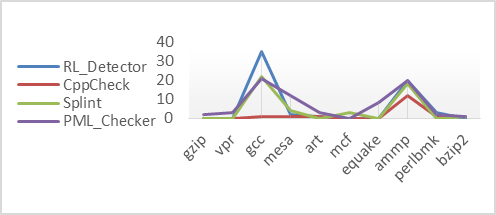
\includegraphics[width=0.45\textwidth]{figure/fig8-fig12/fig10}
\caption{The MLF of each tool on SPEC CPU 2000}
\label{fig:10}
\end{figure}

\begin{figure}[!h]
\center
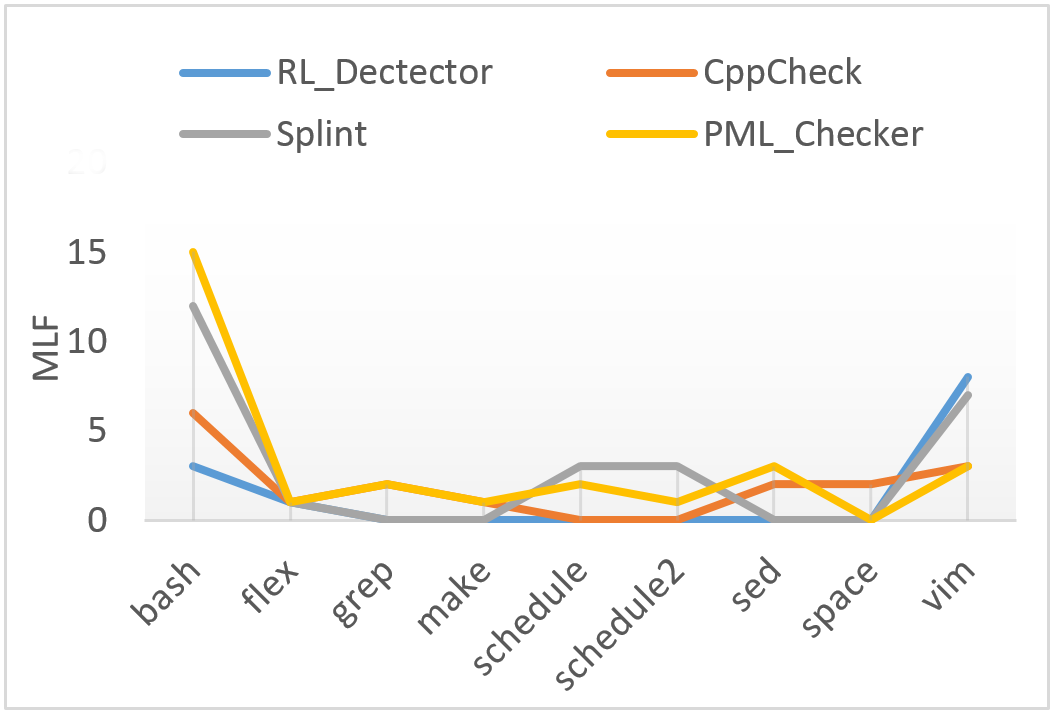
\includegraphics[width=0.45\textwidth]{figure/fig8-fig12/fig11}
\caption{The MLF of each tool on SIR}
\label{fig:11}
\end{figure}

In Fig.~\ref{fig:10}, the abscissa shows the name of the program corresponding to each row in the matrix, the ordinate shows the value of corresponding MLF. This figure displays the number of memory leaks confirmed by manually checking, among the test results on the $15$ programs from SPEC CPU $2000$. We conclude from the figure that the CFG projection has a good detection result on all the test sets except gcc, for the reasons that the program gcc is larger than others in scale. Therefore, we deduce that the scalability of the CFG projection approach for large scale test objects needs to be improved. While in Fig.~\ref{fig:11}, due to the smaller amount of loc(line of code) comparing to SPEC CPU 2000 and fewer \textit{TW} of each tool, the advantage of PML\_Checker is not obvious. But the analysis results between the two benchmarks are generally consistent.

Third, considering symbolic method are used in A1(CppCheck), A3(RL\_Detector) and A4(PML\_Checker), meanwhile, in order to verify whether our approach to influence the running time, so this section chooses SPEC CPU 2000 as the test object due to its large amount of code and large number of files, compared and analyzed run time of the three tools.  Table~\ref{tab:6} lists the run time on this benchmark. Comparing the run time of these three tools, we conclude that the performance of RL\_Detector and PML\_Checker is better than CppCheck in run time, and our approach did not affect the run time of PML\_Checker.

\begin{table}[!h]
\center
\caption{Run time on SPEC CPU $2000$}\label{tab:6}
\hspace{-0.5cm}\begin{tabular}{|c|c|c|c|c|}
\hline
\textbf{Program}& \textbf{Size(Kloc)} & \textbf{A1(s)} & \textbf{A3(s)} & \textbf{A4(s)}\\
\hline
gzip       & 7.8    & 5.3  & 4.5 & 3.2\\
\hline
vpr        & 17.0   & 10.0  & 7.5 & 7.6\\
\hline
gcc        & 205.8 & 167.7  & 48.3 & 41.0 \\
\hline
mesa     & 49.7   & 51.0  & 33.1 & 34.8\\
\hline
art         & 1.3     & 0.3  & 0.9 & 0.4\\
\hline
mcf        & 1.9     & 1.0  & 4.0 & 3.7\\
\hline
equake   & 1.5     & 0.2  & 1.0 & 0.4\\
\hline
crafty     & 18.9   & 27.3	 & 14.2	 & 13.3\\
\hline
ammp    & 13.3   & 7.4 & 10.3 & 10.0\\
\hline
parser    & 10.9   & 4.0	 & 6.7	 & 5.1\\
\hline
perlbmk & 58.2   & 123.2   & 41.3	 & 39.0\\
\hline
gap        & 59.5   &  29.0 & 20.9 & 20.0\\
\hline
vortex    & 52.7    & 73.2	 & 30.1	 & 26.7\\
\hline 
bzip2     & 4.6      & 2.0 & 0.6	 & 1.5\\
\hline
twolf     & 19.7     & 11.0 & 23.7	 & 24.0\\
\hline
Total     & 581.0    & 512.6 & 247.1 & 230.7\\
\hline
\end{tabular}
\end{table}

\noindent\textbf{Experiment on test cases from SARD} 
\\
This experiment analyzed the results of the four tools on test cases from SARD. The \textit{FPR} and \textit{FNR} were measured to the accuracy of different approaches on the same test suite. Table~\ref{tab:7} shows the test results on these test cases, and Fig.~\ref{fig:12} is a histogram that compares test results metrics of the four detection tools. Comparing our approach with other approaches, we have the following observations.

%First, we calculated the false negative rate from the test results of $20$ test cases with memory errors marked ``bad", and the false positive rate from the test results of $20$ test cases without memory errors which corresponding to the ``bad" cases marked ``good". Specifically, \textit{FNR}(RL\_Detector) = 0.7, and \textit{FPR}(RL\_Detector) = 0. \textit{FNR}(CppCheck) = 0.5, and \textit{FPR} (CppCheck) = 0. \textit{FNR}(Splint) = 0.8, and \textit{FPR}(Splint) = 0.05. \textit{FNR}(PML\_Checker) = 0.3, and \textit{FPR}(PML\_Checker) = 0.

The \textit{FPR} of PML\_Checker is the lowest among the four tools. For the analysis of \textit{FPR}, there are no false positives in the results of RL\_Detector, CppCheck and PML\_Checker, while Splint reported a false positive, which confirmed that Splint has a high \textit{FPR} in experiment \RNum{1}. This experiment failed to compare the \textit{FPR} due to the small scale of the programs, but the test results on \textit{FNR} reflected the accuracy of our approach in detecting memory leaks.

\begin{table}[!h]
\center
\caption{Test results on SARD test cases}\label{tab:7}
\begin{tabular}{|c|c|c|c|c|}
\hline
\textbf{Test Cases} & \textbf{A1} (TW)& \textbf{A2} (TW) & \textbf{A3} (TW) & \textbf{A4} (TW)\\
\hline
bad cases(20) &10 & 4 & 6 & 14\\
\hline
good cases(20) & 0 & 	1 &	0 &	0\\
\hline
FPR & 0& 5\% & 0 & 0\\
\hline
FNR & 50\% & 80\% & 70\% & 30\%\\
\hline
\end{tabular}
\end{table}

\begin{figure}[!h]
\center
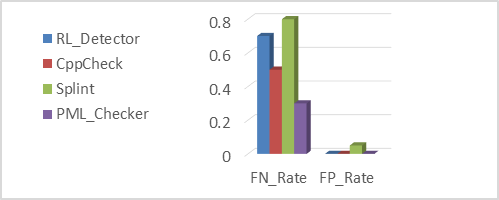
\includegraphics[width=0.45\textwidth]{figure/fig8-fig12/fig12}
\caption{The bar chart of test results}
\label{fig:12}
\end{figure}

\subsection{Summary}
From the above experimental results, we have the following main findings including advantages and limitations: 
\begin{itemize}
\item 
For the complex control flows and complex data types analysis, our projection-based approach is better than the other three approaches.
\item 
For the accuracy of detection, our projection-based approach shows a lower false negative rate compared to other tools, while it shows a high false positive rate in some public benchmarks (such as SPEC CPU $2000$ and SIR). Therefore, in the next step, more detailed data flow analysis will be added into our approach.
\item 
For the scalability of detection, our experiment needs to expand the range of detection. Specifically, our system will detect the large scale benchmarks with millions of code lines, or source code from some open source software.
\end{itemize}

%!TEX root = bare_conf.tex
\section{Related Works}\label{sec:related}

\subsection{Research on Static Approaches to Memory Leaks}
%Currently, the common approaches~\cite{YZ04} used in static memory detection include type inference\footnote{Type inference. https://en.wikipedia.org/wiki/Type\_inference. 2017.}, rule-based inspection~\cite{SJP05}, and symbolic execution followed by constraint solving. However, all these approaches have limitations when dealing with large scale programs. Type inference automatically derives the type of variables by tools, this approach is suitable for analyzing large scale programs, but it is not applicable to the control flow analysis. Regarding rule-based inspection, its scalability is poor due to that describing a program into rules is complicated and error-prone. For symbolic execution, the number of paths will increase exponentially with the increase of the program size, which leads to problems such as ``path-explosion" and ``infinite-search-space", and thus increases the time complexity of entire detection. Comparing to the above approaches, CFG based approach simplifies paths and avoids the ``path-explosion" during symbolic execution. Besides, static detection tools still to be improve in other places, such as ~\cite{JSHB13}, it discusses this issue from developer's perspective.

In recent years, some researchers proposed new static approaches to memory leak detection. \cite{XZX11},~\cite{XZX15} and~\cite{HL06} detect errors by model checking. \cite{XZX11},~\cite{XZX15} proposed Memory State Transition Graph (MSTG) and implemented the tool -- Melton. While ~\cite{HL06} considered from the perspective of object ownership and modeling it. But these approaches may cause high positive rate in some cases. \cite{DWC12} presented heap memory abstract method for heap-manipulating programs. For complex programs, our approach show higher accuracy at detecting memory leaks.   

We also survey the static detection tools particularly for memory leaks detection. Noted that one tool may adopt multiple approaches. We highlight some well-known tools as follows. One of them is Prefix~\cite{BPS00}, which is embedded in the Visual Studio. Prefix detects memory leaks by symbolic simulation. It is path-sensitive and uses function summaries for scalability. However, Prefix explores one path at a time, which becomes inefficient when procedures have many paths. %Heuristics limit the search to a small set of paths. 
Some other tools show a high analysis accuracy by using different techniques. For instance, Splint and CppCheck use the rule-based approach, where Splint mainly analyzes style and annotations of program, and CppCheck detects errors by matching expressions. As an example of flow-sensitive approach, tool Cqual\footnote{Cqual. http://www.cs.umd.edu/~jfoster/cqual/. 2004.} uses type inference and constraint solving techniques for improve accuracy. These tools essentially check the potential memory leaks by adding annotations for the access operation in the source programs. This approach has high preciseness, however, it will generate many false positives as the complexity of the program increases, because the annotations added cannot be reused. Tool RL\_Detector~\cite{J14} detects resource leaks in C programs. It improves detection efficiency by constructing resource behavior to streamline slices, this method retains all statements that are allocated and deallocated of resources, as well as the statements that affect the use of the resource (including memory). Our tool is based on~\cite{XA05,YZ04}, and combines approaches such as symbolic execution, which are used in the above tools as well. Compared with existing work, our tool is specific for detecting memory leaks in C programs, especially in the program with complex control flows. 

\subsection{Research on Complex Programs Analysis}
%\subsection{Regarding the Complex Control Flow Concept}
%There are few studies on complex control flow in the field of static analysis. As in~\cite{KJMP06}, this concept is mainly used in the process of dynamic testing to predict some frequently executed paths, in order to eliminate false positive caused by the evaluating the conditional branches. In~\cite{KK12}, the concept is only used to show a method to measure the complexity of programs, which is irrelevant to memory detection. %in complex control flows. 
There is almost no memory leak detection research for complex control flow.~\cite{KJMP06, KFM13} study control flow graphs. The DMP(diverge-merge processor) in~\cite{KJMP06} is a processor architecture to predict complex branches dynamically.~\cite{KFM13} presents a method to calculate all the worst paths from any node. There are other studies on complex object-oriented programs like~\cite{LLQ16, MGDD14}. Specifically, the research object of~\cite{LLQ16} are complex path conditions, and the research object of~\cite{MGDD14} are inheritance and friend functions in object-oriented languages.~\cite{KK12} shows a method to measure the complexity of programs.

\subsection{Research on Projection in Program Analysis}
%In the field of program analysis, especially in the detection of program dynamic memory leaks, the researchers are more inclined to adopt the dynamic memory modeling methods. For example, \cite{KK16} builds a heap abstraction model that restrains the heap model by combining multiple abstraction positions into a summary position, however in practical applications, there is still a great gap on accuracy between the results of this method and the exact results. \cite{WJG14} builds a pointer behavior model, this model utilizes model checking tools to verify the reachability of assertions to analyzing memory leaks. \cite{MFS12} builds a bounded model, where the memory leaks properties are added. This method transforms the memory leaks problem into solving satisfiability problem, thereby achieves the memory leaks detection. However, this detection scheme needs to reduce the generated verification space and accordingly improve the accuracy of verify. Our approach builds a program model, which is used to be traversed and stored into the stack following some rules for detecting memory leaks.

Recently, the idea of projection is often applied to computer vision~\cite{DG14, HWS15}, mathematical model selection~\cite{NL10} and other related research fields due to its close relationship with graphs. There are only a few of papers use the projection method in the program analysis. \cite{D94} analyzes the specification and abortion of programs by the projection of functions. While in terms of security, this paper only takes a conservative analysis, in other words, the output is ``uncertain” or ``unknown” for some uncertain input, which is relatively fuzzy, so the accuracy of the analysis results need to be improved. In our approach, we redefine the projection of the program control flow graphs, and solve safety problems with a specific algorithm for detecting memory leaks.

%!TEX root =  bare_conf.tex
\section{Conclusion}\label{sec:conclusion}

In this paper, we focus on memory leak detection with complex control flows. We propose a projection-based approach to increase the accuracy in detecting memory leaks in C source code. We implement a detection tool named PML\_Checker, and evaluate our approach by comparing with three open-source tools (CppCheck, Splint, RL\_Detector) on real-world repositories (SPEC CPU $2000$, SIR), public benchmarks (SARD) and CC code. Experimental results show that our approach has lower false negatives than three other approaches, especially in C source code with complex control flows and complex data types. The future direction is to improve our approach in terms of scalability. Specifically, it is possible to improve the detection accuracy by combining with other static methods such as data flow analysis.


\bibliographystyle{IEEEtran}
\bibliography{Mdetection}

\end{document}

\bibliography{Mdetection}
